\documentclass[11pt]{article}

\usepackage[utf8]{inputenc}
\usepackage[T1]{fontenc}
\usepackage{lmodern}
\usepackage{amsmath,amssymb}
\usepackage[numbers,round]{natbib}
\usepackage{booktabs}
\usepackage{graphicx}
\usepackage{geometry}
\usepackage[expansion=false]{microtype}
\usepackage[hidelinks]{hyperref}
\usepackage{setspace}
\usepackage{lineno}
\geometry{letterpaper,margin=1in}
\doublespacing
\linenumbers

\newcommand{\salvi}{\textit{Snodgrassella alvi}}
\newcommand{\demodex}{\textit{Demodex}}

\title{Closed-reference $k$-mer cross-mapping fabricates a \salvi{} rosacea
signal that dissolves under amplicon-sequence-variant resolution}
\author{Jonathan Reich \\
  {\small Independent Researcher, Melbourne, Victoria, Australia} \\
  {\small Corresponding author: \texttt{jonathanreich100@gmail.com}} \\
  {\small ORCID: \href{https://orcid.org/0009-0000-0108-0717}{0009-0000-0108-0717}}}
\date{}

\begin{document}
\maketitle

\begin{abstract}
\demodex{} mites are strongly associated with rosacea, motivating a shortcut:
could the relative abundance of \demodex-associated bacteria in a
routine 16S amplicon sample act as a non-invasive proxy for mite burden? We test
this on public data and, critically, stress-test our own positive result. We
audited the Sequence Read Archive (656
runs, 25 BioProjects; 17 on-topic), assembled a panel of \demodex-associated taxa
(\salvi{}, \textit{Bacillus oleronius}, \textit{Cutibacterium kroppenstedtii},
\textit{Bartonella quintana}), and built a background-subtracted, closed-reference
$k$-mer index. On a paired ivermectin arm (6 subjects) the index did not move
(all $p \ge 0.25$). On an ocular \demodex-versus-control arm (14 versus 17) with a
body-site-matched negative control, the composite separated the groups in the
predicted direction (ROC-AUC $0.66$), apparently carried by \salvi{}. We then
resolved that lead to exact sequences with a DADA2 pipeline and SILVA v138.1
taxonomy. It did not survive:
\emph{none} of $8{,}551$ amplicon sequence variants (ASVs) is
\textit{Snodgrassella}, and our own \salvi{} diagnostic $k$-mers map only onto
commensal Neisseriaceae ($92$--$94\%$ identity to the \salvi{} reference)---a
conserved-region cross-mapping artefact. The strongest exact-sequence association
is a single \textit{Neisseria} ASV enriched on infected surfaces
(AUC $0.70$; nominal one-sided $p=0.032$), which we present as a
hypothesis-generating lead. We conclude that closed-reference marker counting is
not species-specific on short 16S and can fabricate a genus-level signal that
only ASV resolution exposes, and that a surface microbiome cannot grade
individual mite burden---direct mite quantification remains the basis for
treatment.
\end{abstract}

\section*{Importance}
Rosacea is a common, distressing facial skin disease linked to overgrowth of
\demodex{} mites. A bacterial swab that could estimate a patient's mite load
would be clinically attractive, sparing an invasive skin biopsy. Reanalysing
public sequencing data, we show why this shortcut fails and surface a broader
cautionary lesson. A fast, popular way of naming bacteria from short DNA
reads---closed-reference counting---appeared to detect a mite-associated
bacterium, \salvi{}, separating affected from healthy ocular surfaces. At
single-nucleotide resolution that bacterium was absent: the signal came from
unrelated common bacteria sharing a conserved DNA stretch. Microbiome studies
that name species this way risk reporting organisms that are not present unless
they confirm hits at exact-sequence resolution. The one signal that withstood
scrutiny---a \textit{Neisseria} variant---offers a sharper, testable lead for how
the skin community tracks \demodex{}.

\section{Introduction}

The mite \demodex{} folliculorum colonises the human pilosebaceous unit, and its
density is markedly elevated in rosacea: a meta-analysis of 23 case--control
studies put the odds ratio for infestation at roughly nine
\citep{chang2017}, and several authors argue the mite is causal rather than
incidental \citep{forton2020}. A coherent mechanism links the mite to the
disorder's canonical inflammatory axis: \demodex{} and its bacterial passengers
stimulate Toll-like receptor 2 and drive cathelicidin/LL-37 production
\citep{yamasaki2007}, placing the mite upstream of the very inflammation that
the standard neurovascular/innate-immune account foregrounds. The strongest
therapeutic evidence on the ``it is the organism'' side is that a purely
antiparasitic agent, topical ivermectin, reduces inflammatory lesions and
outperforms metronidazole \citep{steingold2014,taieb2015}, and its benefit
tracks changes in the skin bacterial community as mite density falls
\citep{nakatsuji2025}.

If mite burden is the driver, then quantifying it should guide therapy: heavier
antiparasitic cover for high-density infestation, lighter where the load is low.
The reference assay is the standardised skin-surface biopsy with mite counting,
which is labour-intensive and operator-dependent. This motivates a tempting
shortcut. The mite carries a recognisable bacterial cargo---\salvi{}, an
insect-gut symbiont, was recovered from a heavily \demodex-colonised facial
sample in a recent multi-omic study \citep{olah2025}, \textit{Bacillus
oleronius} antigens stimulate inflammatory cells in rosacea \citep{lacey2007},
and \textit{Cutibacterium kroppenstedtii} and \textit{Bartonella quintana} have
been tied to the mite or to papulopustular rosacea, whose flora also shifts under
antibiotic therapy \citep{murillo2014,rainer2020,woo2020}---and these bacteria
appear in ordinary
16S amplicon surveys. Could their summed relative abundance act as a molecular
proxy for mite load?

We answer with a deliberately austere, fully reproducible test, and we hold our
own result to the standard the field often skips: when the closed-reference index
produced a positive marker signal, we re-derived it at amplicon-sequence-variant
(ASV) resolution to check whether it was real. It was not. The headline is
therefore twofold---a methodological caution (closed-reference $k$-mer counting
can manufacture a species-level signal from conserved 16S) and a relocated lead
(the genuine \demodex-associated variant at the ocular surface is
\textit{Neisseria}, not \salvi{})---and we argue both halves are useful precisely
because the first nearly fooled us.

\section{Data and methods}

\subsection{Data-availability audit}
Using NCBI E-utilities we searched the Sequence Read Archive and BioProject for
rosacea/\demodex{} sequencing, recovering 656 runs across 25 BioProjects, of
which 17 were on-topic (Table~\ref{tab:audit}). Because the BioProject
\texttt{esummary} endpoint was returning a server-side error during the study
window, study-level metadata were recovered from the SRA side via
\texttt{efetch}. Two datasets anchor the analysis: a topical-ivermectin
before/after facial-skin 16S series (PRJDB18292; 6 subjects $\times$ \{lesional,
non-lesional\} $\times$ \{pre, post\}) and a \demodex-infection-versus-control
ocular-surface 16S series (PRJNA692647; 14 vs 17).

\begin{table}[t]
\centering
\small
\begin{tabular}{llr l}
\toprule
BioProject & marker & $n$ & description \\
\midrule
PRJDB18292   & 16S & 24 & topical ivermectin, before/after (facial) \\
PRJEB82826   & multi & 96 & rosacea multi-omics (infestation + microbiome) \\
PRJNA1189573 & 16S & 93 & skin/blood/stool microbiome in rosacea \\
PRJNA856121  & WGS & 72 & ocular \demodex{} metagenomics \\
PRJNA879945  & 16S & 42 & \demodex{} blepharitis, treatment \\
PRJNA692647  & 16S & 31 & \demodex{} infection vs control (ocular) \\
\bottomrule
\end{tabular}
\caption{Representative on-topic BioProjects from the SRA audit (17 total).
``multi'' = multi-omic; ``WGS'' = shotgun.}
\label{tab:audit}
\end{table}

\subsection{\demodex-associated taxon panel and diagnostic $k$-mers}
For each panel taxon we fetched up to eight 16S references from NCBI and computed
the set of canonical 31-mers. A $k$-mer is deemed \emph{diagnostic} for a taxon
if it occurs in that taxon's references but in (i) no other panel taxon and
(ii) none of a background set of common human flora. The background subtraction
is essential: without it, conserved 16S stretches shared with abundant flora are
misattributed to rare \demodex-associated taxa, inflating the signal by one to
two orders of magnitude. Crucially the background must be \emph{matched to the
body site}: a skin-only background (24 facial taxa) leaves ocular samples open to
cross-mapping, so for the ocular cohort we extended it with ocular/environmental
and Rhizobiales/\textit{Bacillus} relatives (38 taxa total). Two abundant skin taxa
(\textit{Cutibacterium acnes}, \textit{Staphylococcus epidermidis}) are carried
as scored context but excluded from the \demodex{} index.

\subsection{The molecular mite-burden index}
For each sequencing run we streamed the FASTQ from the European Nucleotide
Archive, decompressed it in flight, and attributed a read to a taxon when it
carried at least two diagnostic $k$-mers for that taxon (the two-hit rule raises
specificity over single-$k$-mer attribution). The per-taxon score is the
fraction of reads so attributed; the composite \texttt{mite\_index} is the sum of
the four \demodex-associated fractions. The index is an explicitly relative,
closed-reference proxy---not an ASV census.

\subsection{Statistics}
Treatment effects used the paired Wilcoxon signed-rank test and an exact sign
test within subject$\times$site strata ($n=6$ pairs). Group separation used the
Mann--Whitney $U$ test (two-sided and the one-sided \demodex{}$>$control
alternative) and the ROC-AUC obtained from the $U$ statistic. The $k$-mer steps are
pure-Python with offline self-tests; networked steps are read-only and cached.

\subsection{Exact-sequence (ASV) re-analysis}\label{sec:dada2}
To test the closed-reference lead at single-nucleotide resolution we reprocessed
the ocular cohort (PRJNA692647) with a faithful DADA2 pipeline
\citep{callahan2016}. The runs are paired-end $2\times250$ V4 (515F/806R)
mislabelled \texttt{SINGLE} in the archive; primers (preceded by a variable
heterogeneity spacer) were removed with \texttt{cutadapt} \citep{martin2011},
after which \texttt{filterAndTrim} (truncation $170/150$, \texttt{maxEE}$=2$),
\texttt{learnErrors}, \texttt{dada}, \texttt{mergePairs}, and
\texttt{removeBimeraDenovo} yielded amplicon sequence variants. Taxonomy used the
SILVA v138.1 training set with exact-match species assignment \citep{quast2013}.
To bridge the two methods we applied the \emph{same} diagnostic $k$-mer panels
directly to the ASV sequences (two-hit rule) and computed the percent identity of
each flagged ASV to its panel taxon's 16S reference. ASV group separation used
the same Mann--Whitney $U$/AUC as above.

\section{Results}

\subsection{Specificity must be engineered, not assumed}
The first, unbackground-subtracted index attributed 20--50\% of reads to
\textit{Bacillus oleronius} and \textit{Bartonella}---biologically impossible for
rare commensals---because panel-unique $k$-mers still fell in conserved 16S
regions shared with the dominant skin flora. Subtracting a 24-taxon skin
background and requiring two diagnostic $k$-mers per read collapsed these to
plausible levels (single digits to low hundreds of reads), with the dominant
signal correctly residing in \textit{C. acnes}/\textit{S. epidermidis}. This is
a cautionary methods result in its own right: closed-reference marker counting
on short 16S reads is only as good as its negative control.

\subsection{Treatment arm: null and mixed}
Across the paired ivermectin design, neither the composite index nor any single
\demodex-associated taxon changed significantly from pre- to post-treatment in
either lesional or non-lesional skin (all $p \ge 0.25$; Table~\ref{tab:treat}).
The direction was mixed (four up, two down for the lesional composite), with one
subject dominating the variance. We read this as a sampling-physics result more
than a biological one: surface swabs under-sample a mite that lives deep in the
follicle, and antiparasitic-induced mite lysis can transiently release bacterial
cargo onto the surface, so a surface bacterial readout is a poor instrument for a
follicular load.

\begin{table}[t]
\centering
\small
\begin{tabular}{lrrrr}
\toprule
stratum & $n$ & down/up & median $\Delta$ & Wilcoxon $p$ \\
\midrule
lesional / composite     & 6 & 2/4 & $+0.0006$ & 0.84 \\
non-lesional / composite & 6 & 2/4 & $+0.0008$ & 0.69 \\
\bottomrule
\end{tabular}
\caption{Ivermectin before/after (PRJDB18292): paired tests on the composite
mite index. No stratum or single taxon reached significance.}
\label{tab:treat}
\end{table}

\subsection{Validation arm: the verdict turns on the negative control}
In the \demodex-versus-control comparison the answer depends on whether the
background is matched to the body site. With a \emph{skin-only} background the
composite did not discriminate (ROC-AUC $0.41$); decomposition showed why
\textit{Bartonella} ran backwards (AUC $0.30$), a near-certain artefact of
cross-mapping to ocular Proteobacteria (Rhizobiales/Alphaproteobacteria) absent
from that background. We therefore extended the background with ocular and
environmental taxa and with Rhizobiales/\textit{Bacillus} relatives of the panel.
This collapsed the artefact (the \textit{Bartonella} diagnostic set fell from
$1244$ to $776$ $k$-mers and its per-sample reads from thousands to single
digits), and re-scoring gave a different verdict (Table~\ref{tab:val}): the
composite now separates infected from control surfaces in the predicted direction
(AUC $0.66$; one-sided $p \approx 0.074$), carried by \salvi{} (AUC $0.65$;
$p \approx 0.085$) and \textit{Bacillus} (AUC $0.58$). \textit{Bartonella} is
still faintly inverted but now contributes essentially nothing (median
$4.6\times10^{-5}$), so it no longer drags the sum. The methodological moral is
blunt: closed-reference marker counting on short amplicons is meaningless
without a body-site-matched negative control, and the Stage-1 ``failure'' was an
artefact of a mismatched one---not evidence against the \demodex{} hypothesis.
We stress, however, that this $k$-mer attribution is provisional: Sec.~\ref{sec:asv}
shows the \salvi{} component is itself a cross-mapping artefact once the reads are
resolved to exact sequences.

\begin{table}[t]
\centering
\small
\begin{tabular}{lrrr}
\toprule
metric & median (dem) & median (ctl) & AUC (dem$>$ctl) \\
\midrule
composite mite index          & 0.02430 & 0.01952 & \textbf{0.66} \\
\salvi{}                      & 0.00535 & 0.00398 & 0.65 \\
\textit{Bacillus oleronius}   & 0.01717 & 0.01541 & 0.58 \\
\textit{C. kroppenstedtii}    & 7.3e$-$5 & 8.7e$-$5 & 0.43 \\
\textit{Bartonella quintana}  & 4.6e$-$5 & 7.2e$-$5 & 0.28 \\
\bottomrule
\end{tabular}
\caption{\demodex{} infection vs control (PRJNA692647), \emph{body-site-matched
background}: group medians and ROC-AUC for the one-sided \demodex{}$>$control
alternative. With a skin-only background the composite instead gave AUC $0.41$
(Bartonella cross-mapping); see text.}
\label{tab:val}
\end{table}

\begin{figure}[t]
\centering
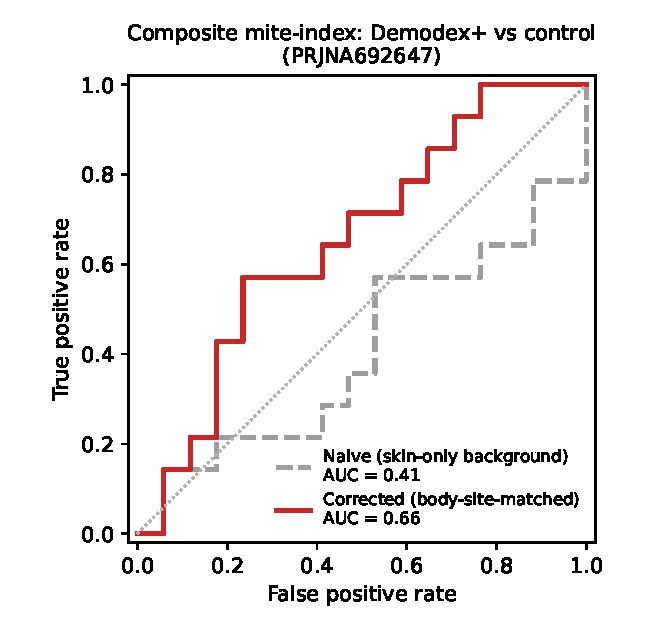
\includegraphics[width=0.55\textwidth]{results/fig_roc_validation.pdf}
\caption{ROC curves for the composite mite index on the \demodex-versus-control
cohort (PRJNA692647). With a skin-only background (naive) the composite is
anti-predictive (AUC $0.41$), driven by \textit{Bartonella} cross-mapping; with
a body-site-matched background (corrected) the same index separates infected
from control surfaces in the predicted direction (AUC $0.66$). The shift is due
entirely to the negative control, not to any change in the scored taxa.}
\label{fig:roc}
\end{figure}

The two regimes are shown in Fig.~\ref{fig:roc}: the curve crosses from below to
above the chance diagonal once the background is matched to the body site.

\subsection{Method characterisation}\label{sec:charac}
To bound the index's resolution we ran a held-out control: for each panel taxon,
sensitivity is the fraction of simulated $250$\,bp windows over \emph{held-out}
same-taxon 16S references (accessions beyond the build set) detected under the
two-hit rule, and specificity is the same applied to congeneric/confamilial
challengers that must not be called. Sensitivity was high ($0.74$--$0.98$), and
the panels were clean against distant relatives ($0.00$ for, e.g.,
\textit{Neisseria gonorrhoeae}, \textit{Bacillus subtilis}, \textit{C.\ acnes},
\textit{Brucella abortus}). However, close congeners cross-reacted
($0.43$--$0.67$ for \textit{Kingella}, \textit{Heyndrickxia},
\textit{C.\ diphtheriae}, and \textit{B.\ henselae}), so the index resolves at
roughly genus level. Although the \salvi{} panel read clean against the single
\textit{Neisseria} reference used here, the ASV analysis (Sec.~\ref{sec:asv})
shows this held-out control was too thin: against the diverse commensal
Neisseriaceae actually present at the ocular surface, the panel cross-maps
freely---a reminder that specificity bounded by a handful of distant challengers
can badly overstate real-world specificity.

\subsection{ASV resolution overturns the marker attribution}\label{sec:asv}
Denoising PRJNA692647 gave $8{,}551$ ASVs ($97.4\%$ of reads retained, ${\sim}94\%$
of pairs merged, length mode $253$\,bp). The closed-reference lead did not
survive. \emph{No} ASV is classified as \textit{Snodgrassella}, although SILVA
v138.1 contains the genus ($25$ references) and Neisseriaceae ($1{,}795$), so this
is genuine absence rather than a reference gap. Applying our own \salvi{}
diagnostic $k$-mer panel directly to the ASVs flags only \emph{non-Snodgrassella}
Neisseriaceae---\textit{Neisseria}, \textit{Eikenella}, \textit{Uruburuella},
\textit{Bergeriella}---plus \textit{Methylotenera}/\textit{Psychrobacter}; the
top-hit ASVs are $92.5$--$94.5\%$ identical to the \salvi{} 16S reference over
V4, an inter-genus distance, not the ${\approx}99\%$ expected for true \salvi{}.
The Stage-2 ``\salvi{}'' signal was therefore conserved-region cross-mapping onto
abundant commensal Neisseriaceae. The same exercise shows the \textit{Bacillus}
panel cross-maps across Bacillota (\textit{Anoxybacillus}, \textit{Enterococcus},
\textit{Geobacillus}, \textit{Oscillibacter}) and the \textit{Bartonella} panel
onto Rhizobiaceae---confirming, at sequence level, the artefacts that background
subtraction only partly contained.

What \emph{does} survive is sharper than the original claim: a single exact
\textit{Neisseria} ASV (the most abundant Neisseriaceae variant, $4{,}367$ reads)
is enriched on \demodex-infected surfaces with AUC $0.70$ (nominal one-sided
$p=0.032$, uncorrected)---the strongest exact-sequence separation we observed.
The best genuine Bacillaceae variant is weak (AUC $0.64$, $p=0.09$). The ocular
\demodex-associated signal thus relocates from \salvi{} to \textit{Neisseria}.
Notably this does not corroborate the facial \salvi{} observation of
\citet{olah2025}, consistent with the difference in body site, though we caution
that both are single-sample/single-cohort observations.

\section{Discussion}

Three conclusions follow. First, the central methodological lesson: a
closed-reference $k$-mer (or any marker-counting) index on short 16S reads is not
species-specific, and can \emph{manufacture} a plausible genus-level signal. Our
composite appeared to separate \demodex-infected from control surfaces
(AUC $0.66$), apparently carried by \salvi{}; yet at exact-sequence resolution no
\textit{Snodgrassella} is present at all, and the ``\salvi{}'' reads are
conserved-region cross-mapping onto commensal Neisseriaceae ($92$--$94\%$ identity
to the \salvi{} reference). Background subtraction and a held-out specificity
control---both of which we applied---were \emph{not} sufficient to prevent this;
only ASV-level denoising exposed it. \demodex--microbiome association studies that
rely on closed-reference assignment without exact-sequence (ASV/oligotyping)
resolution are therefore at material risk of false species-level findings
\citep{callahan2017}.

Second, the surface-proxy idea fails on its own terms regardless: the index does
not track antiparasitic treatment, and even the (artefactual) group signal was
borderline. A surface microbiome cannot grade an individual's mite burden;
grading should rest on direct mite quantification (the standardised skin-surface
biopsy).

Third, what survives exact-sequence analysis is a sharper, relocated lead: a
single \textit{Neisseria} ASV is enriched on \demodex-infected ocular surfaces
(AUC $0.70$, nominal one-sided $p=0.032$). Because this comparison is post-hoc,
uncorrected, and drawn from one cohort, we present it not as a confirmed
association but as a hypothesis-generating, exact-sequence lead that we are not
aware of being reported previously. A curated, ASV-based \textit{Neisseria} assay
with follicle-targeted sampling is the experiment this analysis now recommends.

The broader moral mirrors null-model design in molecular evolution: an instrument
must encode the structure it claims to measure, and its specificity must be
tested against the diversity actually present, not a handful of distant
challengers. A closed-reference count on short amplicons is only as trustworthy as
the exact-sequence analysis that audits it.

\paragraph{Limitations.} The ASV re-analysis (Sec.~\ref{sec:asv}) resolves the
$k$-mer index's genus-level ambiguity but carries its own caveats: the
\textit{Neisseria} lead rests on a single cohort ($14$ vs $17$) and one dominant
ASV, and the group $p=0.032$ is nominal (uncorrected for the ASVs screened). The
treatment arm is small ($n=6$ pairs), and the validation cohort is \emph{ocular}
rather than facial, so the \textit{Neisseria} association may be specific to the
ocular surface. The facial multi-omic cohort that would adjudicate this
(PRJEB82826, $n=96$, cyanoacrylate follicle sampling; the cohort of
\citet{olah2025}) carries no infestation/clinical labels in its public records,
so a labelled, ASV-level facial validation is blocked pending the authors' sample
key---the natural next step once obtained. Finally, taxonomy rests on SILVA
v138.1; a different reference could rename, though not resurrect, the absent
\textit{Snodgrassella}.

\paragraph{Reproducibility.} The discovery pipeline (audit, panel construction,
index, and analyses) is pure-Python with per-module offline self-tests; the
confirmatory ASV re-analysis is a documented DADA2/R workflow (Sec.~\ref{sec:dada2}).
All networked calls are read-only and cached, and every accession, intermediate
table, $k$-mer panel, and ASV output is released so that all numbers above
regenerate from a clean checkout.

\appendix

\section{Reproducibility and data access}\label{app:repro}

\paragraph{Design goal.} The discovery pipeline (audit, panel, index, statistics)
runs on a stock Python interpreter with no bioinformatics toolchain: all
networking uses the standard library (\texttt{urllib.request}, \texttt{gzip}),
and \texttt{matplotlib} is used only for the figure, keeping it auditable
line-by-line. The confirmatory ASV step (Sec.~\ref{sec:dada2}) deliberately
departs from this austerity: it uses the reference implementation DADA2
(Bioconductor/R) with \texttt{cutadapt} and SILVA v138.1, precisely so that the
audit of our own positive result rests on the community-standard tool rather than
a bespoke one. The two-method contrast is the point---the lightweight index
proposes, and the gold-standard ASV pipeline disposes.

\paragraph{Retrieval (read-only).} Dataset discovery and reference sequences come
from NCBI E-utilities (\texttt{esearch}/\texttt{efetch}) and per-project run
tables from the EBI ENA \texttt{filereport} API, each fetched as a plain HTTPS
\texttt{GET}. During the study window the BioProject \texttt{esummary} endpoint
returned a server-side error, so study-level metadata were recovered from the SRA
side via \texttt{efetch}; the fallback is encoded in the audit script rather than
applied by hand.

\paragraph{Streaming architecture.} Sequencing reads are never downloaded to
disk. For each run, the gzipped FASTQ is opened as an HTTPS response object and
wrapped \emph{in place} by \texttt{gzip.GzipFile}, so the file is decompressed
on the fly while it streams and is consumed four lines (one read) at a time. Peak
memory is therefore a single read plus the in-memory $k$-mer panel, independent
of file size, and no large local storage is required. Each run is retried up to
three times on transient network failures; runs that never succeed are reported
and skipped rather than silently dropped.

\paragraph{Attribution.} The panel is a dictionary mapping each diagnostic
canonical 31-mer (and its reverse complement) to a taxon; a read is attributed
when it carries at least two diagnostic $k$-mers for a taxon. Diagnostic sets are
built by set difference against (i) the other panel taxa and (ii) a
body-site-matched background, and are cached as plain text so the index step is
fully offline once the panel exists.

\paragraph{Verification.} Every module carries an offline \texttt{-{}-self-test}
that exercises its core logic (reverse-complement/canonicalisation, FASTA
parsing, $k$-mer attribution, the ROC/AUC computation, and the
sensitivity/specificity detector) without touching the network, so correctness
can be checked with no data present.

\paragraph{Data access.} All inputs are public. The two analysed cohorts are
ENA/SRA \texttt{PRJDB18292} (topical-ivermectin before/after, facial 16S) and
\texttt{PRJNA692647} (\demodex{} infection vs control, ocular 16S); the audit
covered 656 runs across 25 BioProjects. A facial multi-omic cohort with
cyanoacrylate follicle sampling, \texttt{PRJEB82826} ($n=96$, amplicon), is
catalogued but its public records carry no infestation/clinical labels, so it is
not used here. \texttt{PRJNA692647} was additionally reprocessed end-to-end with
DADA2 (Sec.~\ref{sec:dada2}); the resulting ASV table, taxonomy, sequences, and
the $k$-mer/ASV bridge are released alongside the $k$-mer outputs. The pipeline
(audit, panel construction, panel validation, index,
analyses, and this figure), the diagnostic $k$-mer panels, every intermediate
table, and the exact accession lists are released so that all reported numbers
and Fig.~\ref{fig:roc} regenerate from a clean checkout in documented run order.

\section*{Acknowledgements}
I thank Dr Matheen Mohamed (FACD, MPH; East Malvern Dermatology, Melbourne, and
St Vincent's Hospital, Melbourne) for the clinical observations on \demodex{} and
antiparasitic therapy in rosacea that motivated this reanalysis. No external
funding was received for this work, and the author declares no competing
interests.

\section*{Data availability}
All analysed data are public. The two analysed cohorts are ENA/SRA
\texttt{PRJDB18292} (topical-ivermectin before/after, facial 16S) and
\texttt{PRJNA692647} (\demodex{} infection versus control, ocular 16S); the
facial multi-omic cohort \texttt{PRJEB82826} \citep{olah2025} is catalogued but
its public records carry no infestation/clinical labels and so is not analysed
here. Taxonomic assignment used the SILVA v138.1 reference \citep{quast2013}. All
analysis code, the diagnostic $k$-mer panels, intermediate tables, and the DADA2
ASV table, taxonomy, representative sequences, and $k$-mer/ASV bridge outputs are
openly available at
\url{https://github.com/JohnnyTeutonic/rosacea-demodex-16S-reanalysis} and will
be archived with a permanent DOI (Zenodo) upon acceptance.

\begin{thebibliography}{99}
\bibitem{chang2017} Chang Y-S, Huang Y-C. Role of \demodex{} mite infestation in
  rosacea: a systematic review and meta-analysis. \textit{J Am Acad Dermatol}.
  2017;77(3):441--447.
\bibitem{forton2020} Forton FMN. The pathogenic role of \demodex{} mites in
  rosacea: a potential therapeutic target already in erythematotelangiectatic
  rosacea? \textit{Dermatol Ther (Heidelb)}. 2020;10(6):1229--1253.
\bibitem{yamasaki2007} Yamasaki K, Di Nardo A, Bardan A, et al. Increased serine
  protease activity and cathelicidin promotes skin inflammation in rosacea.
  \textit{Nat Med}. 2007;13(8):975--980.
\bibitem{steingold2014} Stein Gold L, Kircik L, Fowler J, et al. Efficacy and
  safety of ivermectin 1\% cream in papulopustular rosacea. \textit{J Drugs
  Dermatol}. 2014;13(3):316--323.
\bibitem{taieb2015} Taieb A, Ortonne JP, Ruzicka T, et al. Superiority of
  ivermectin 1\% cream over metronidazole 0.75\% cream in treating
  papulopustular rosacea. \textit{Br J Dermatol}. 2015;172(4):1103--1110.
\bibitem{nakatsuji2025} Nakatsuji T, Cheng JY, Butcher A, et al. Topical
  ivermectin treatment of rosacea changes the bacterial microbiome of the skin.
  \textit{J Invest Dermatol}. 2025;145(5). doi:10.1016/j.jid.2024.10.592.
\bibitem[Olah et~al.(2025)]{olah2025} Olah P, Reuvers N, Radai Z, et al. Microbe--host interaction
  in rosacea and its modulation through topical ivermectin. \textit{J Invest
  Dermatol}. 2025;145(10):2576--2587.e8.
\bibitem{lacey2007} Lacey N, Delaney S, Kavanagh K, Powell FC. Mite-related
  bacterial antigens stimulate inflammatory cells in rosacea. \textit{Br J
  Dermatol}. 2007;157(3):474--481.
\bibitem{murillo2014} Murillo N, Aubert J, Raoult D. Microbiota of \demodex{}
  mites from rosacea patients and controls. \textit{Microb Pathog}.
  2014;71--72:37--40.
\bibitem{rainer2020} Rainer BM, Thompson KG, Antonescu C, et al.
  Characterization and analysis of the skin microbiota in rosacea: a
  case--control study. \textit{Am J Clin Dermatol}. 2020;21(1):139--147.
\bibitem{woo2020} Woo YR, Lee SH, Cho SH, Lee JD, Kim HS. Characterization and
  analysis of the skin microbiota in rosacea: impact of systemic antibiotics.
  \textit{J Clin Med}. 2020;9(1):185.
\bibitem{callahan2016} Callahan BJ, McMurdie PJ, Rosen MJ, Han AW, Johnson AJA,
  Holmes SP. DADA2: high-resolution sample inference from Illumina amplicon
  data. \textit{Nat Methods}. 2016;13(7):581--583.
\bibitem{martin2011} Martin M. Cutadapt removes adapter sequences from
  high-throughput sequencing reads. \textit{EMBnet J}. 2011;17(1):10--12.
\bibitem{quast2013} Quast C, Pruesse E, Yilmaz P, et al. The SILVA ribosomal RNA
  gene database project: improved data processing and web-based tools.
  \textit{Nucleic Acids Res}. 2013;41(D1):D590--D596.
\bibitem{callahan2017} Callahan BJ, McMurdie PJ, Holmes SP. Exact sequence
  variants should replace operational taxonomic units in marker-gene data
  analysis. \textit{ISME J}. 2017;11(12):2639--2643.
\end{thebibliography}

\end{document}
